\begin{surferPage}[Singularitat A3--]{Una singularitat $A_3^{--}$}
Mirant l'equació
    \[x^4-y^2-z^2=0\]
es veu que aquesta superfície és similar a l'anterior
(una $A_3^{+-}$, amb equació $x^4+y^2-z^2$).
La imatge dessota a l'esquerra mostra les dues superfícies,
$A_3^{--}$ de color groc i $A_3^{+-}$ de color blau.
La secció amb el pla $y=0$ dóna la mateixa corba en els dos casos:
    \vspace*{-0.5em}
    \begin{center}
      \begin{tabular}{c@{\qquad}c}
        \begin{tabular}{@{}c@{}}
          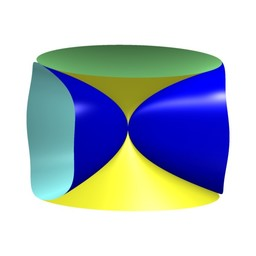
\includegraphics[width=1.6cm]{../../common/images/A3pmA3mm}
        \end{tabular}
        &
        \begin{tabular}{@{}c@{}}
          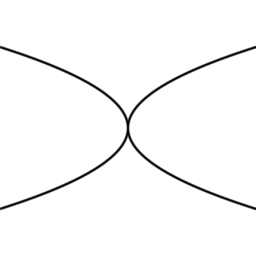
\includegraphics[width=1.6cm]{../../common/images/A3pm_cut}
        \end{tabular}
      \end{tabular}
    \end{center}
    \vspace*{-0.1cm}
Aquesta singularitat $A_3^{- -}$ també es pot deformar en
$2=\lfloor\frac{3+1}{2}\rfloor$ singularitats còniques:
    %
    \begin{center}
      \vspace*{-0.1cm}
      \begin{tabular}{@{}c@{\quad}c@{\quad}c@{}}
        \begin{tabular}{@{}c@{}}
          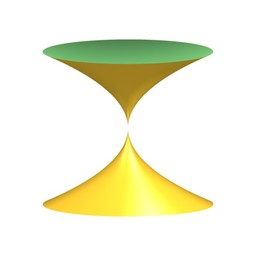
\includegraphics[width=1.6cm]{../../common/images/A3mm_0}
        \end{tabular}
        &
        \begin{tabular}{@{}c@{}}
          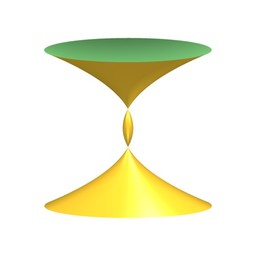
\includegraphics[width=1.6cm]{../../common/images/A3mm_1}
        \end{tabular}
        &
        \begin{tabular}{@{}c@{}}
          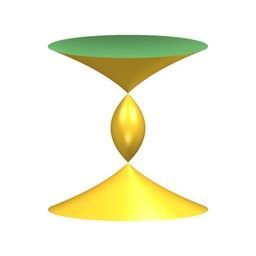
\includegraphics[width=1.6cm]{../../common/images/A3mm_2}
        \end{tabular}
      \end{tabular}
    \end{center}
    \vspace*{-0.2cm}
La deformació de $A_3^{--}$ que es mostra a la imatge
ve donada per l'equació següent:
    \[\bigl(x-\frac12 a^2\bigr)^2\bigl(x+\frac12 a^2\bigr)^2-y^2-z^2.\]
 
\end{surferPage}
